\chapter{Results}

The three SLAM algorithms were evaluated regarding the computed trajectories, the resulting pointclouds and
the computational complexity. 

\section{Trajectory Evaluation}

	In order to evaluate the quality of the trajectory computed by the algorithms, the trajectory firstly had to be 
	transformed into the world reference of the ground truth data. This is because the algorithms usually initialize
	the origin with the first (key)frame and the groundtruth data doesn't. Furthermore, monocular visual slam algorithms 
	are generally not capable to extract the true scale. The alignment was performed using the method of Umeyama, described
	in the \ref{comp} section. 
	After alignment, as a first indicator for the accuracy of the computed trajectories, the trajectories were visually observed by 
	plotting the true position and the evaluated position into a coordiante system. The x, y and z axis were observed seperatly. 
	
	% results here
	
	In figure \ref{fig:flight_path} the computed trajectories are displayed for sequences MH01, V102 and V203. 
	
	% and here 

	\begin{figure}%
    \centering
    \subfloat[\centering MH01]{{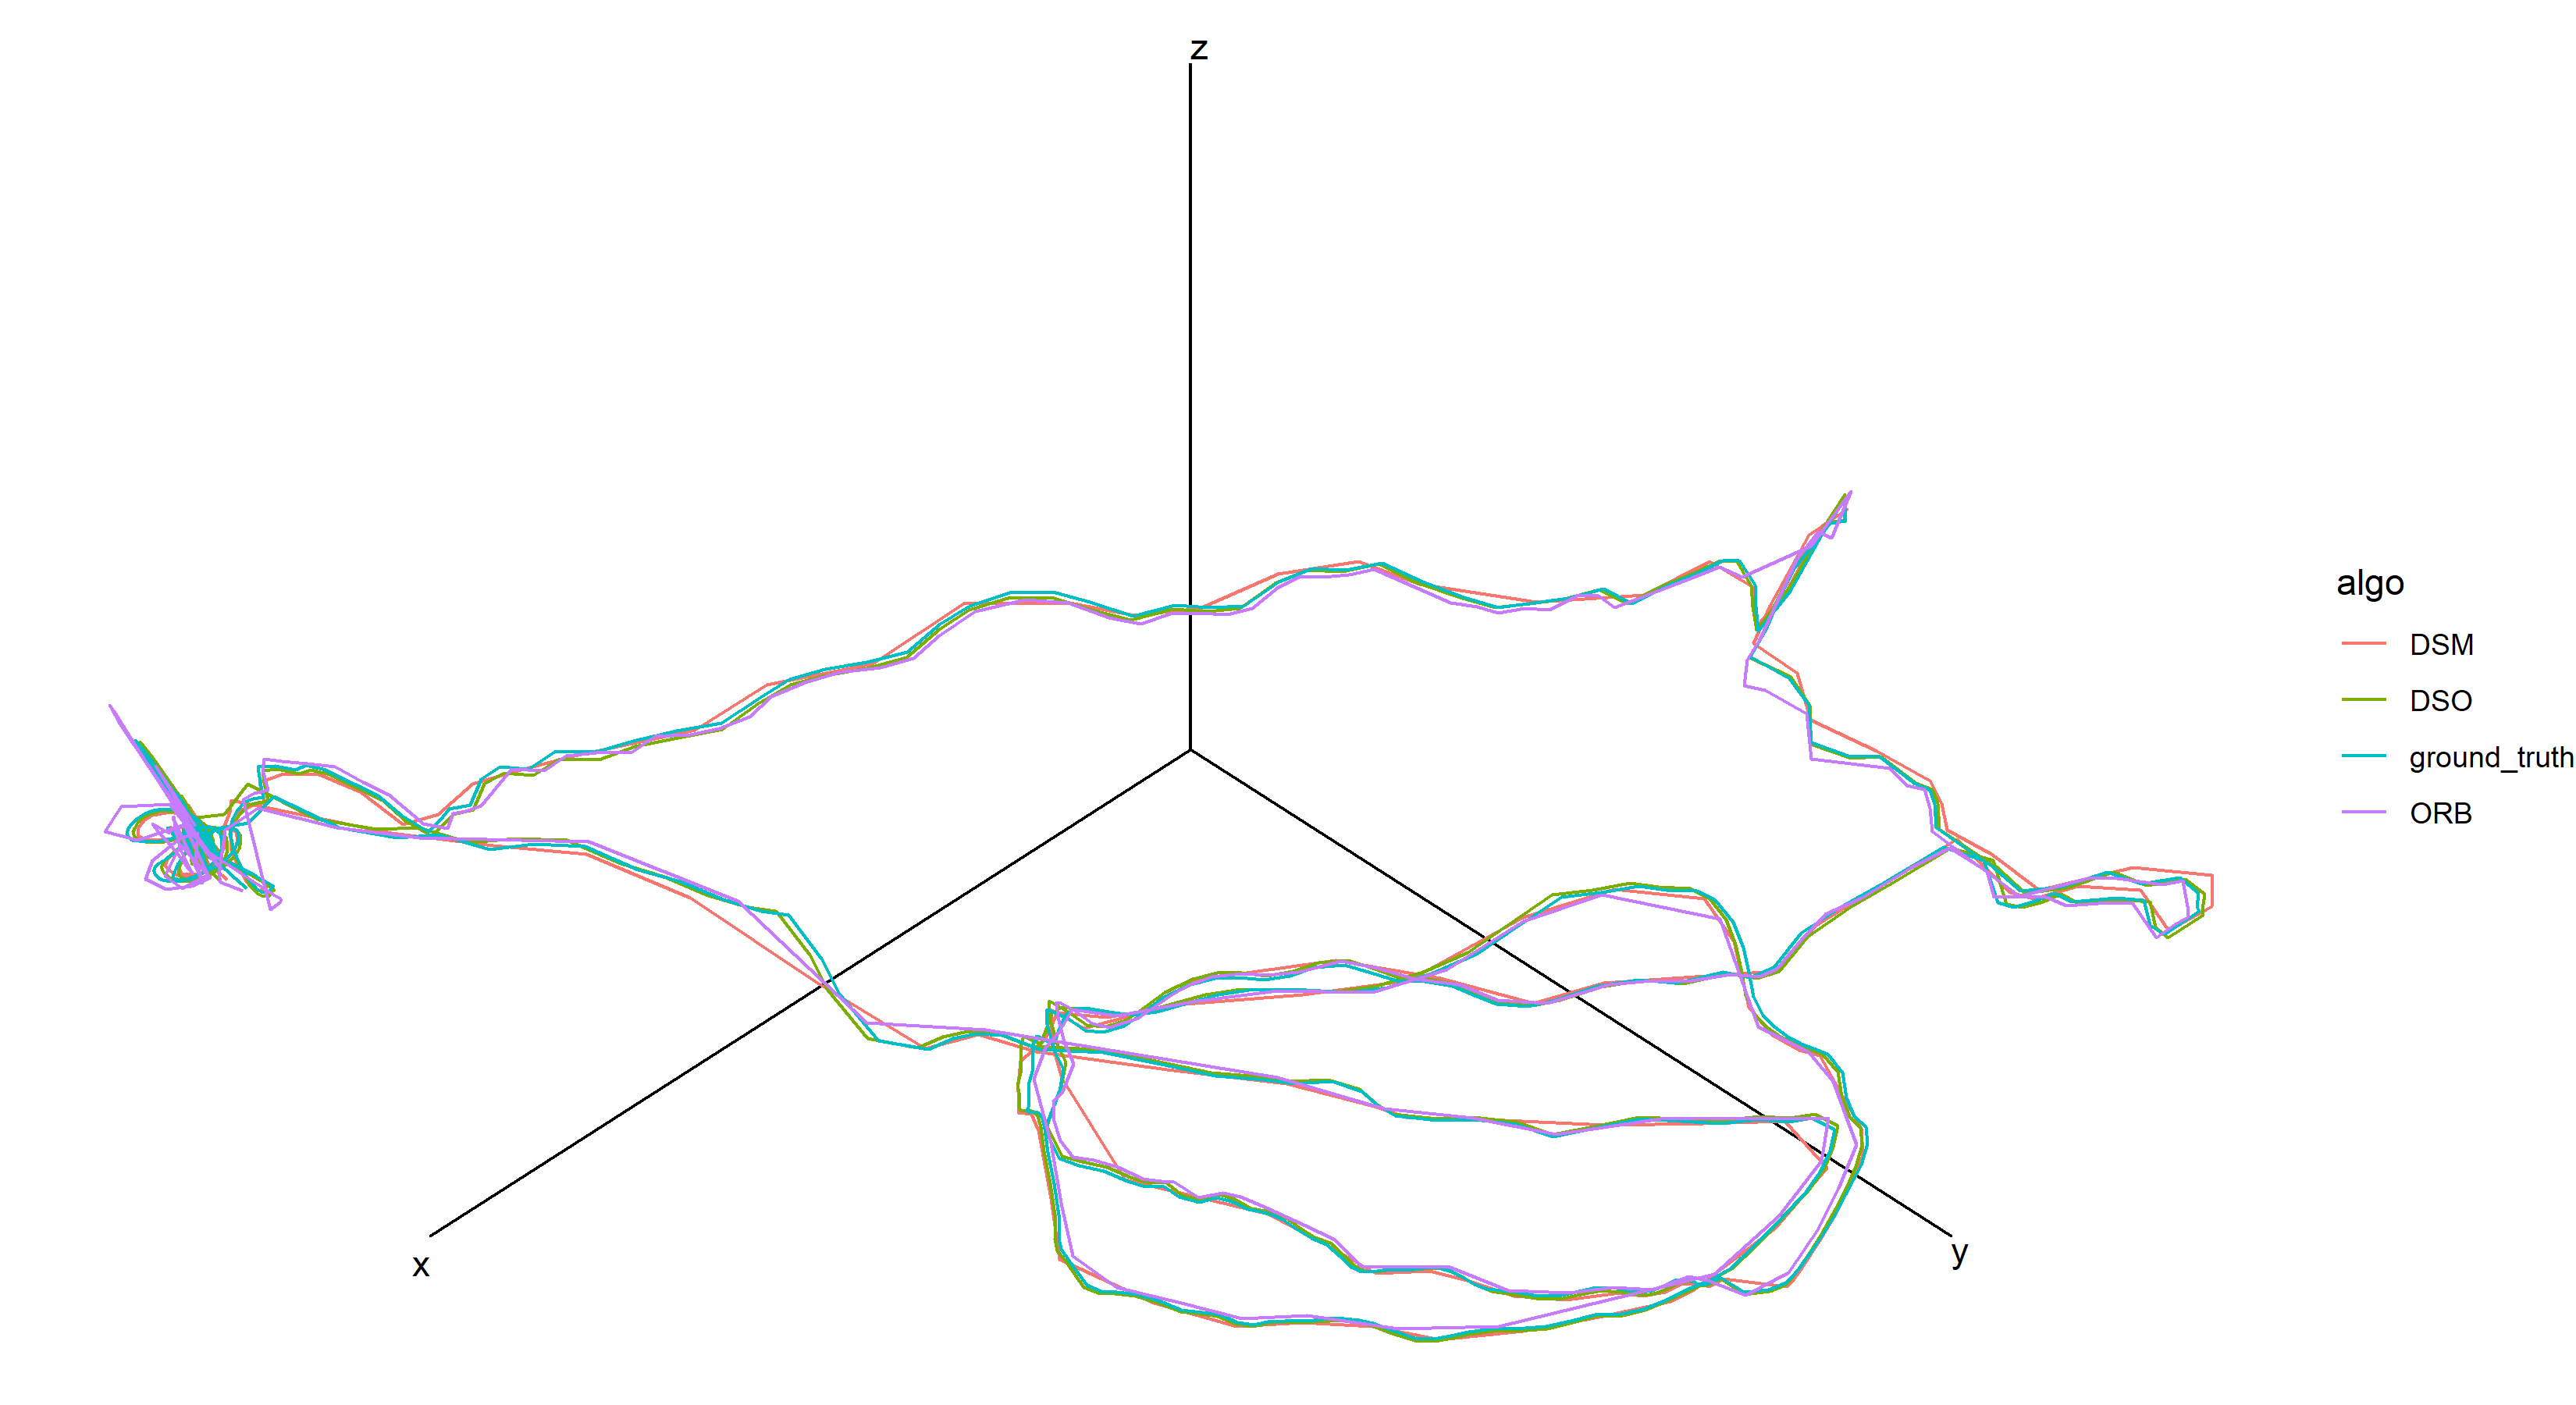
\includegraphics[width=9cm]{img/traj_perf.png} }}%
    \qquad
    \subfloat[\centering V102]{{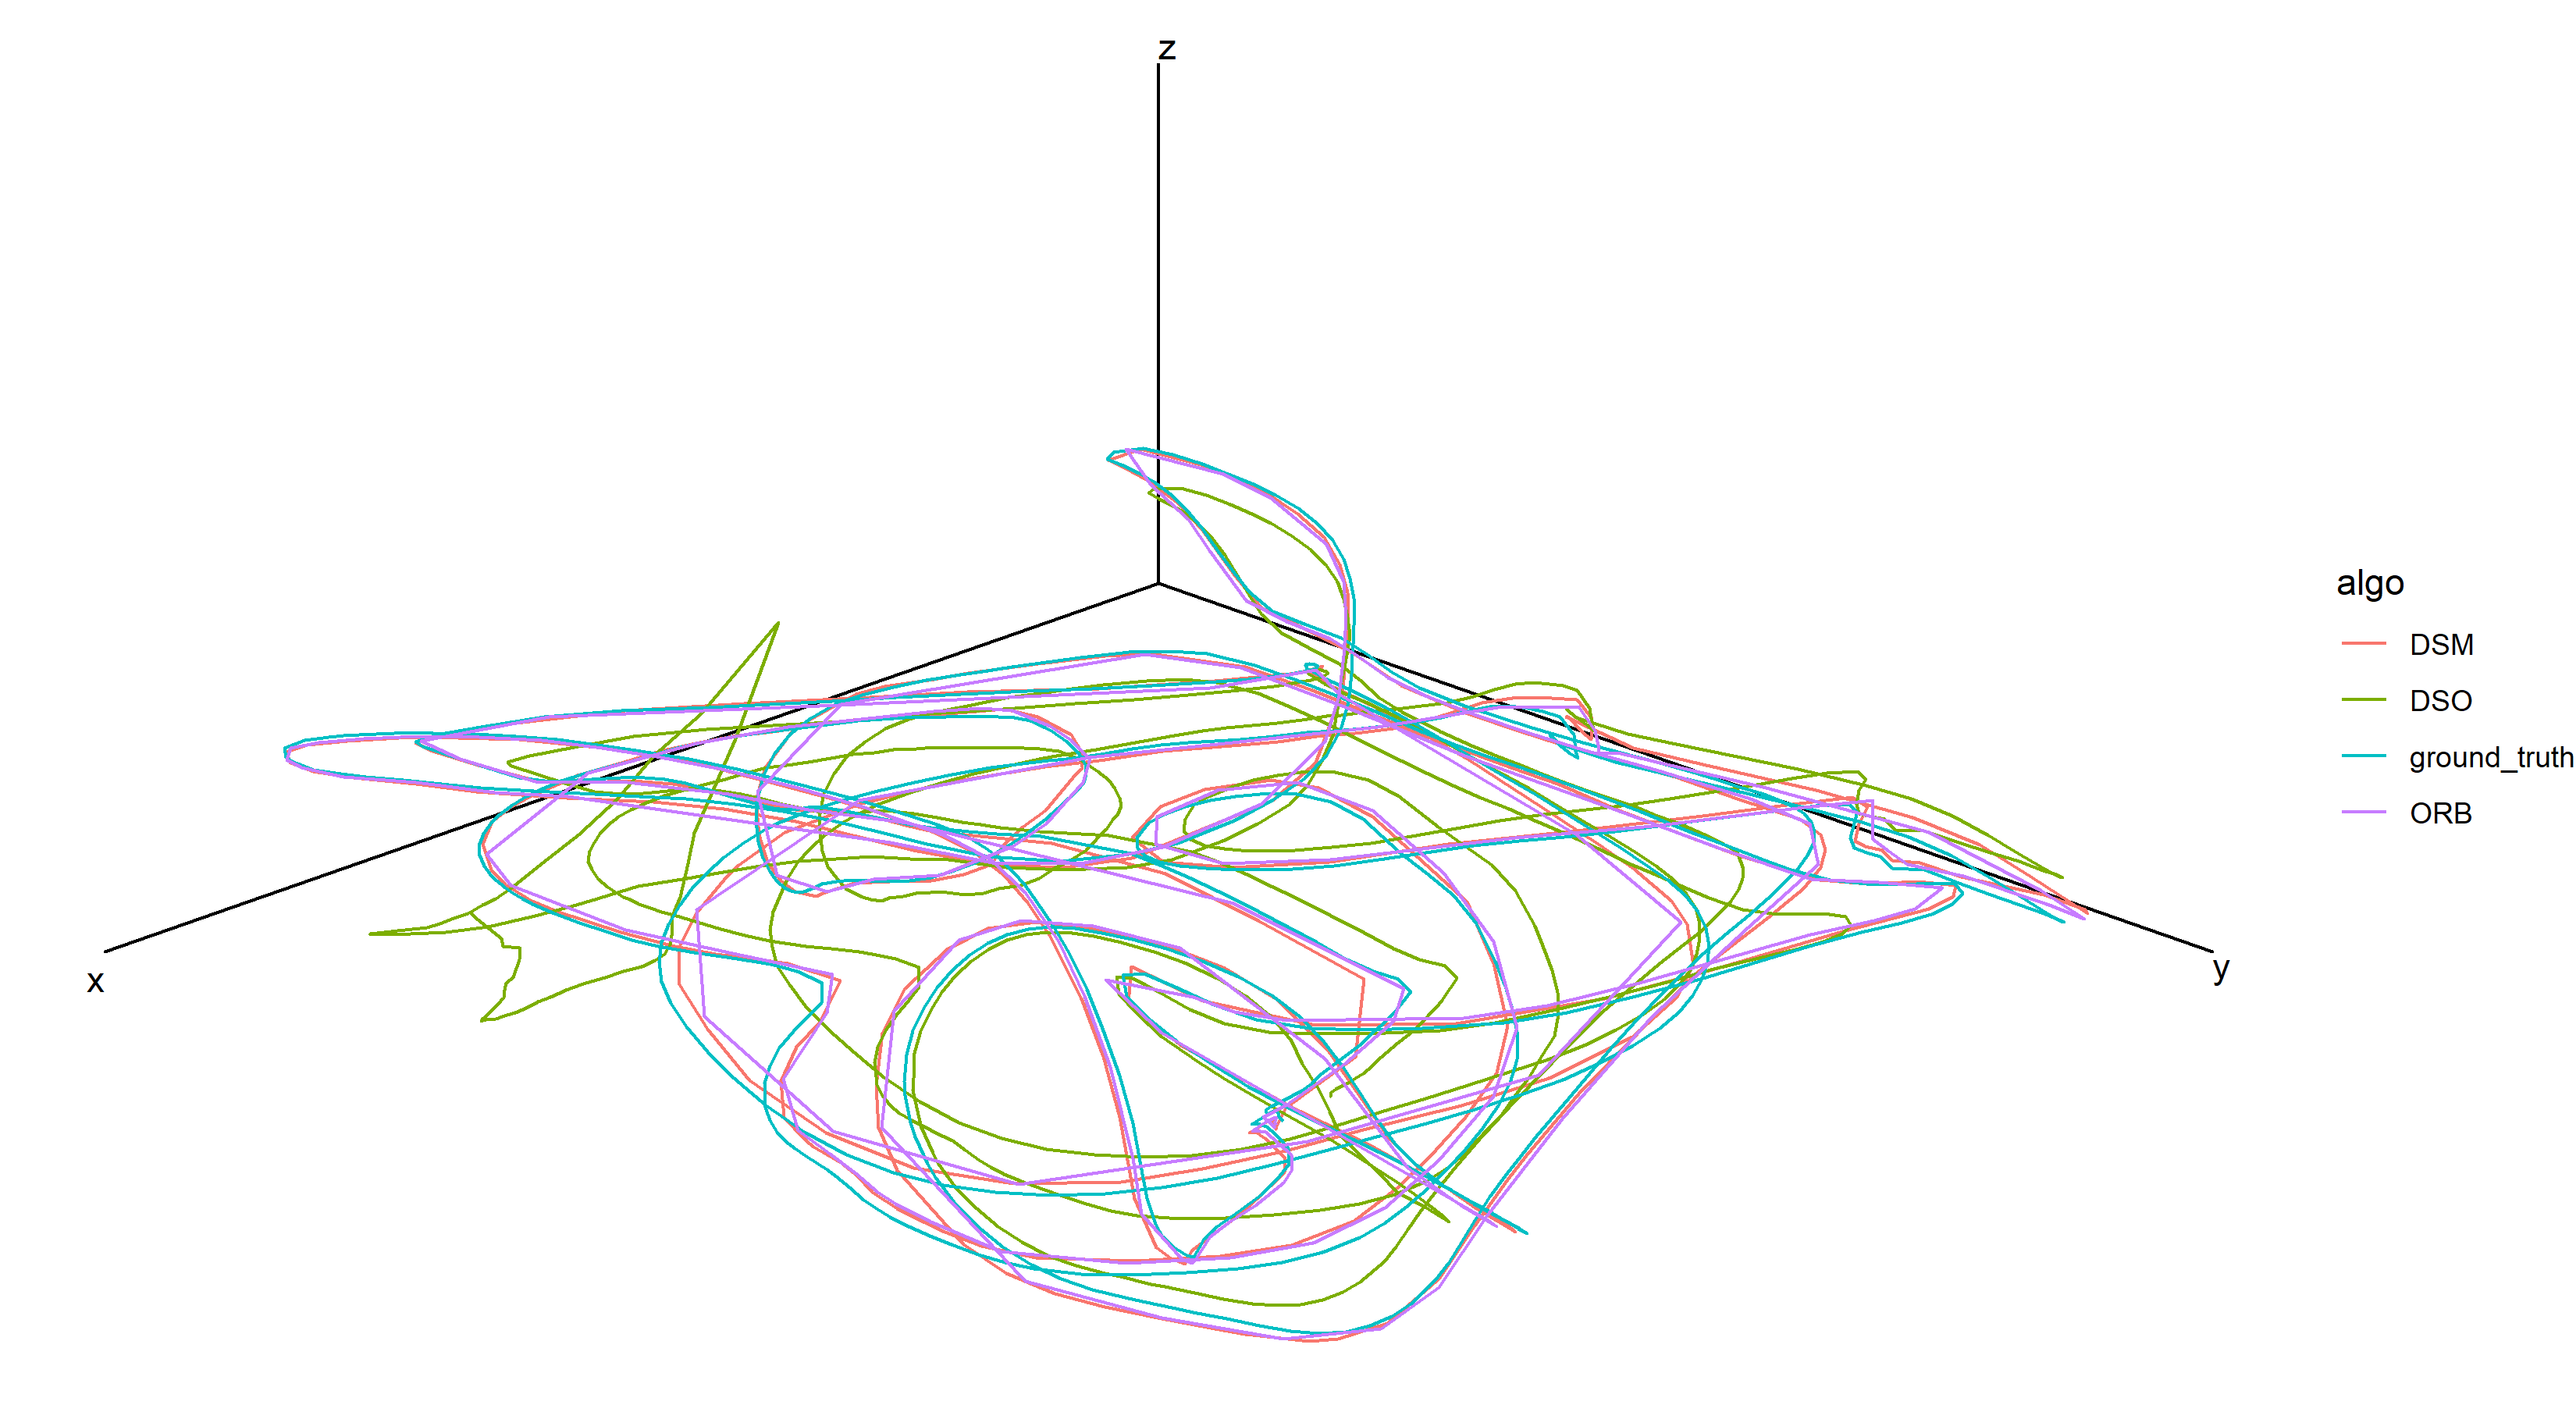
\includegraphics[width=9cm]{img/traj_dso.png} }}%
	\qquad
    \subfloat[\centering V203]{{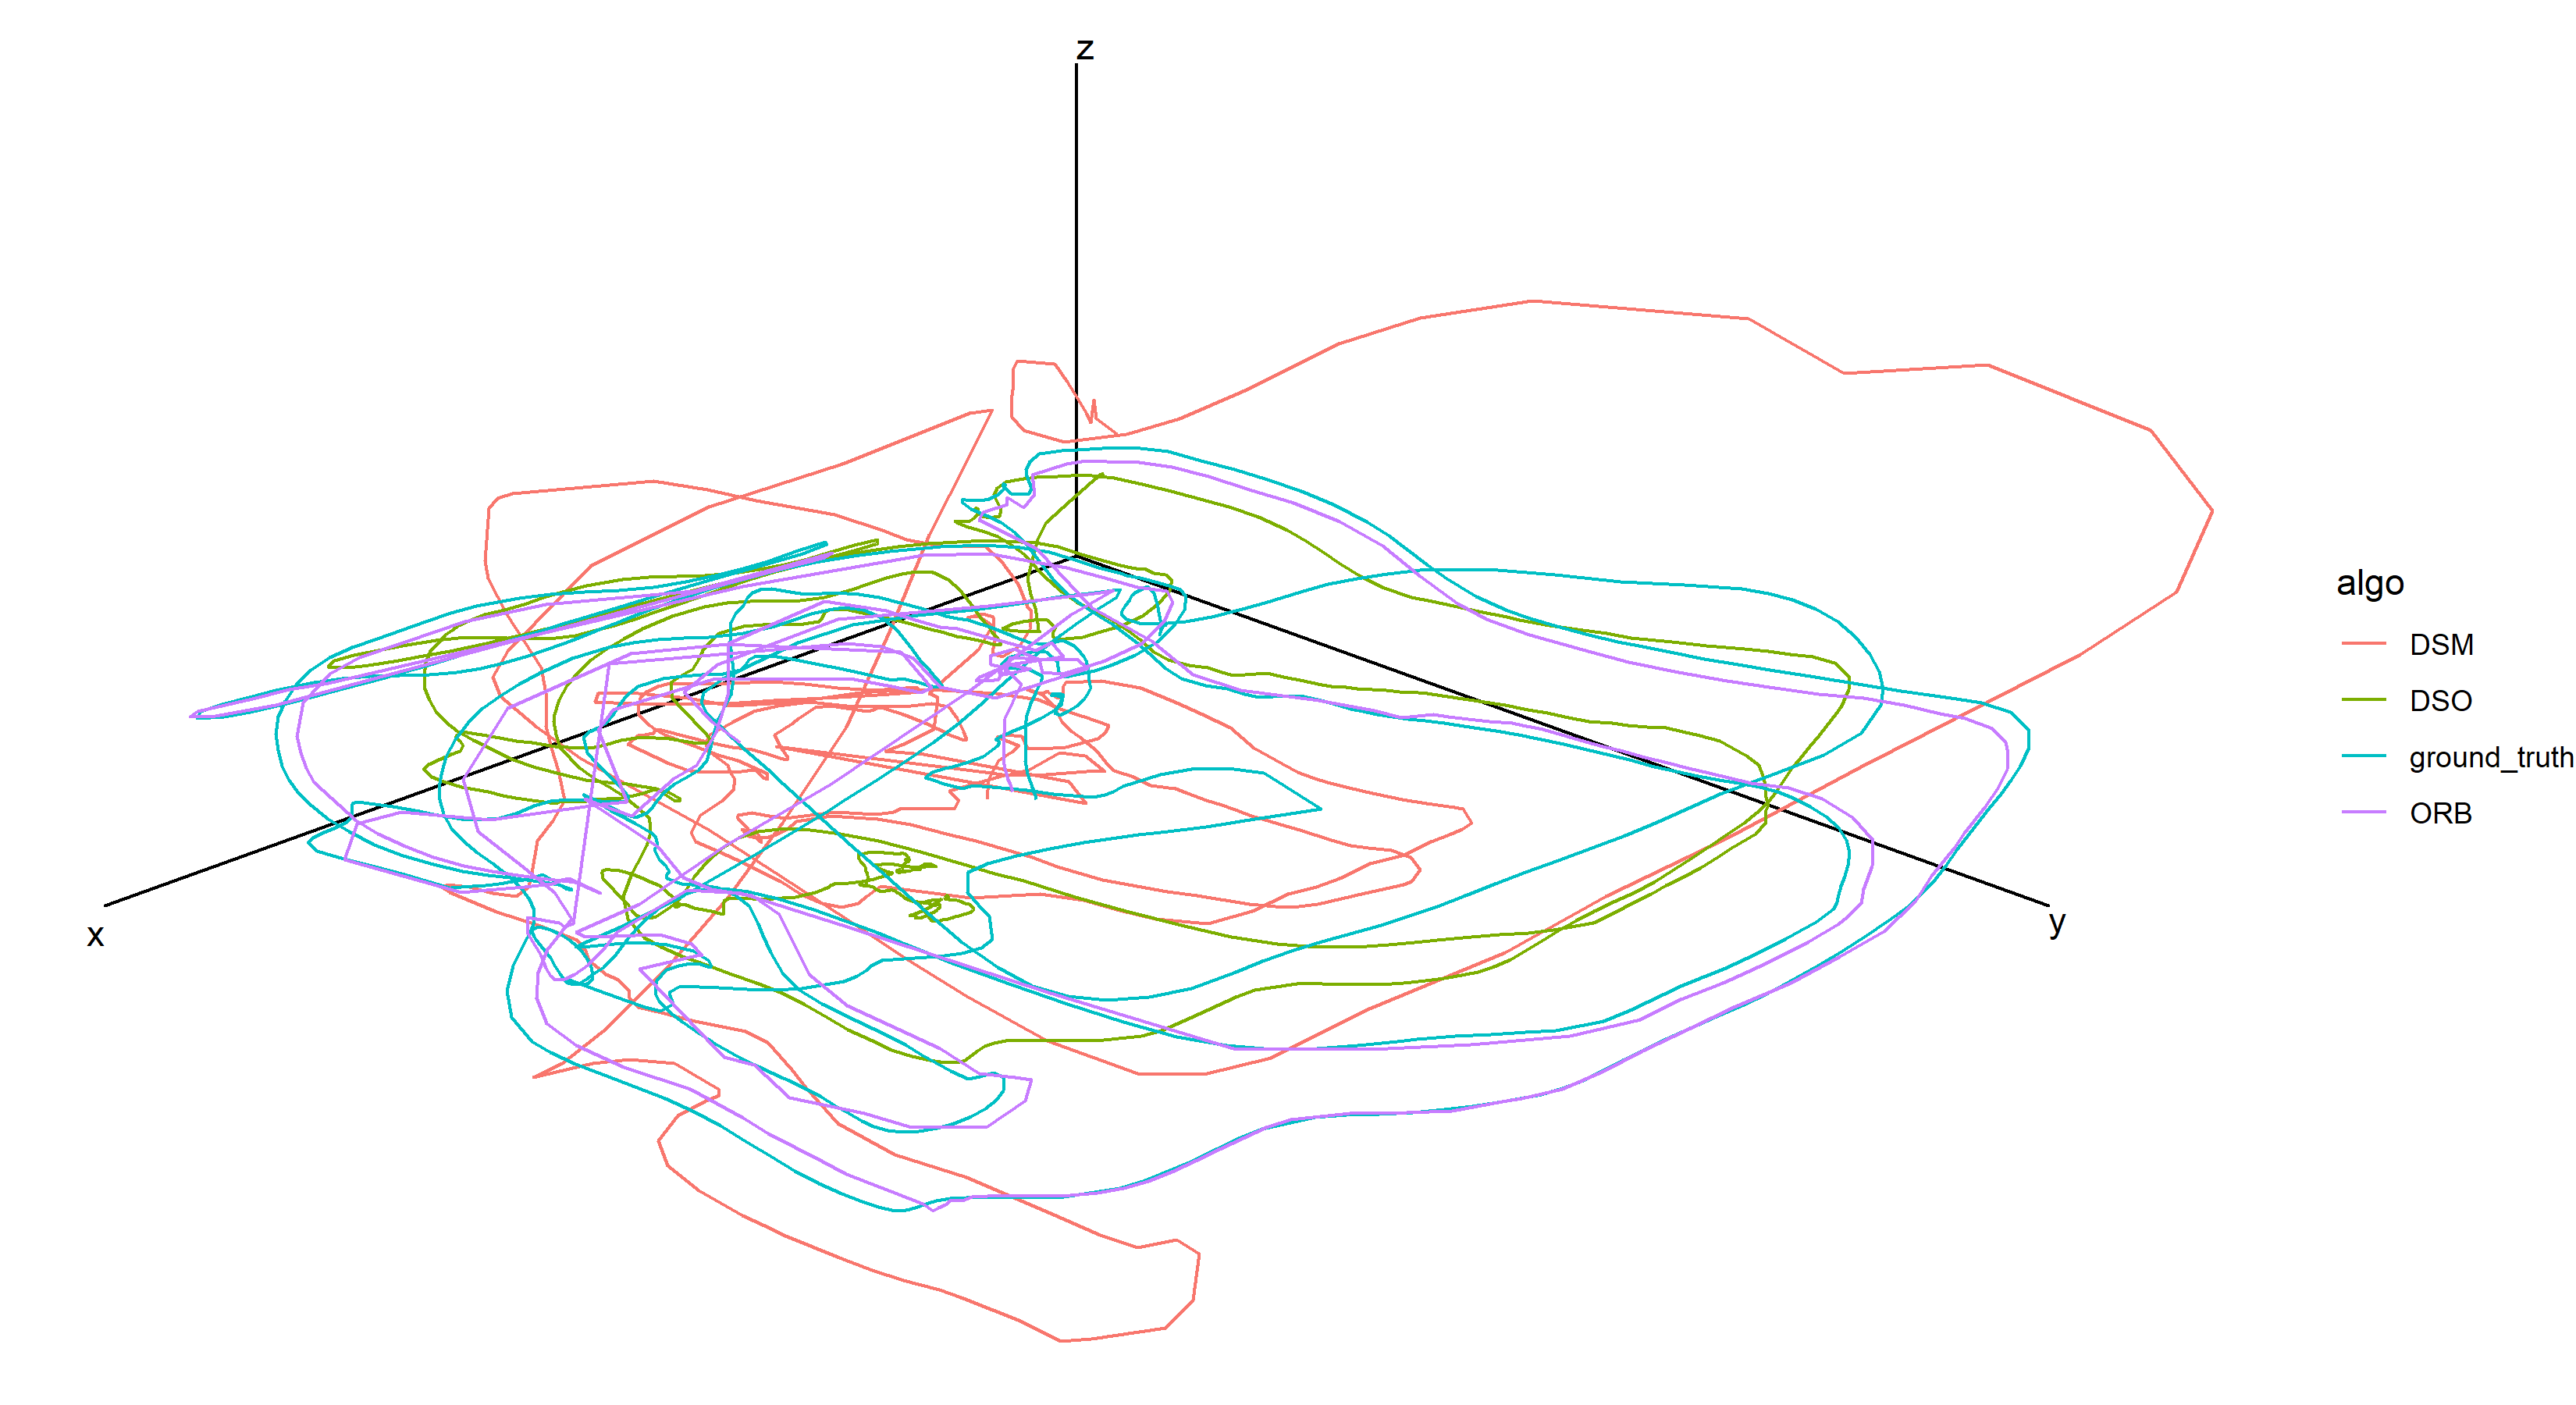
\includegraphics[width=9cm]{img/traj_last.png} }}%
    \caption{
	Ground truth flight path and evaluated flight path of each algorithm after alignment with the method of Umeyama in the x and y axis in meters. 
	Left the sequence MH01, middle the sequence V102 and right the sequence V203 is displyed.
	}%
    \label{fig:flight_path}%
	\end{figure}
	
	
	Furthermore, the eucleadian distances between position of the keyframe and the true postion of the latter are computed. For a keyframe, 
	the entry of the groundtruth data with the lowest distance in time to the time the keyframe was inserted is taken as reference point. 
	This is justifiable, since the true position is sampled at a frequency of over 200 points per second. 
	
	In figure \ref{fig:boxplot_traj} a boxplot of all computed distances over all sequences is displayed. 
	
	% result here. 
	
	
	\fig{img/boxplot_dist.png}{Boxplot of all euclideans distances between the ground truth position of the keyframe and 
	the evaluated position after alignment with the method of Umeyama. Outliers greater than 1.5 are not displayed.
	}{fig:boxplot_traj}{0.8}
	
	
	\fig{img/pos_error.png}{The positional error over time in meters. The vertical lines indicate the beginning of a new sequence}{fig:pos_error}{1}
	


\section{Pointcloud Evaluation}

	\begin{figure}%
    \centering
    \subfloat[\centering ORB]{{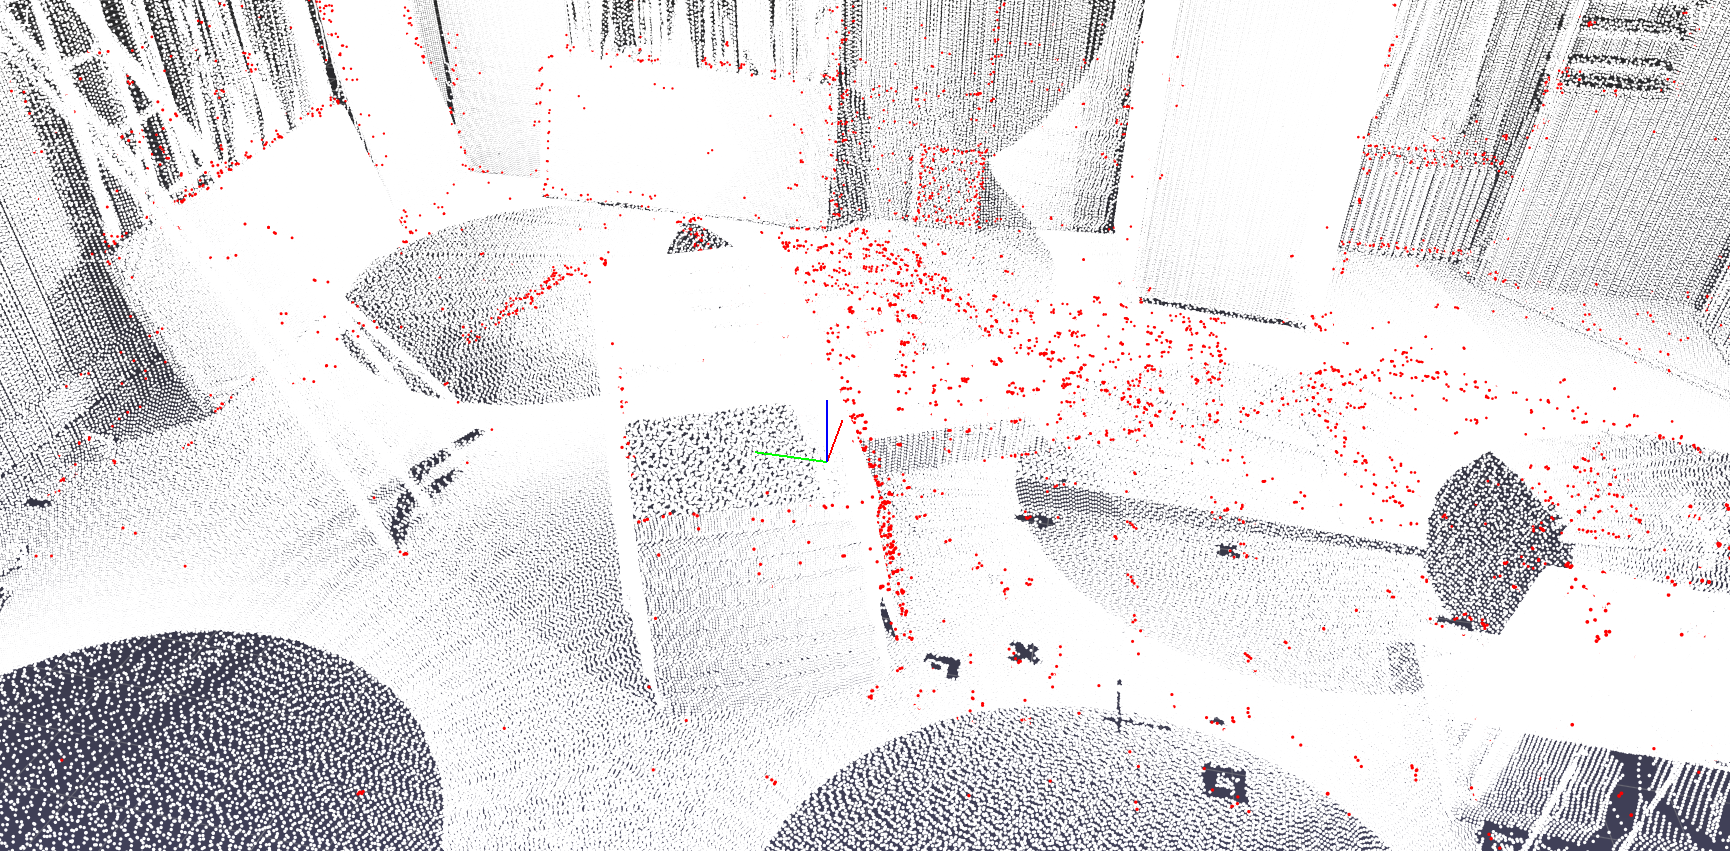
\includegraphics[width=4cm]{img/pointcloud_orb} }}%
    \qquad
    \subfloat[\centering DSM]{{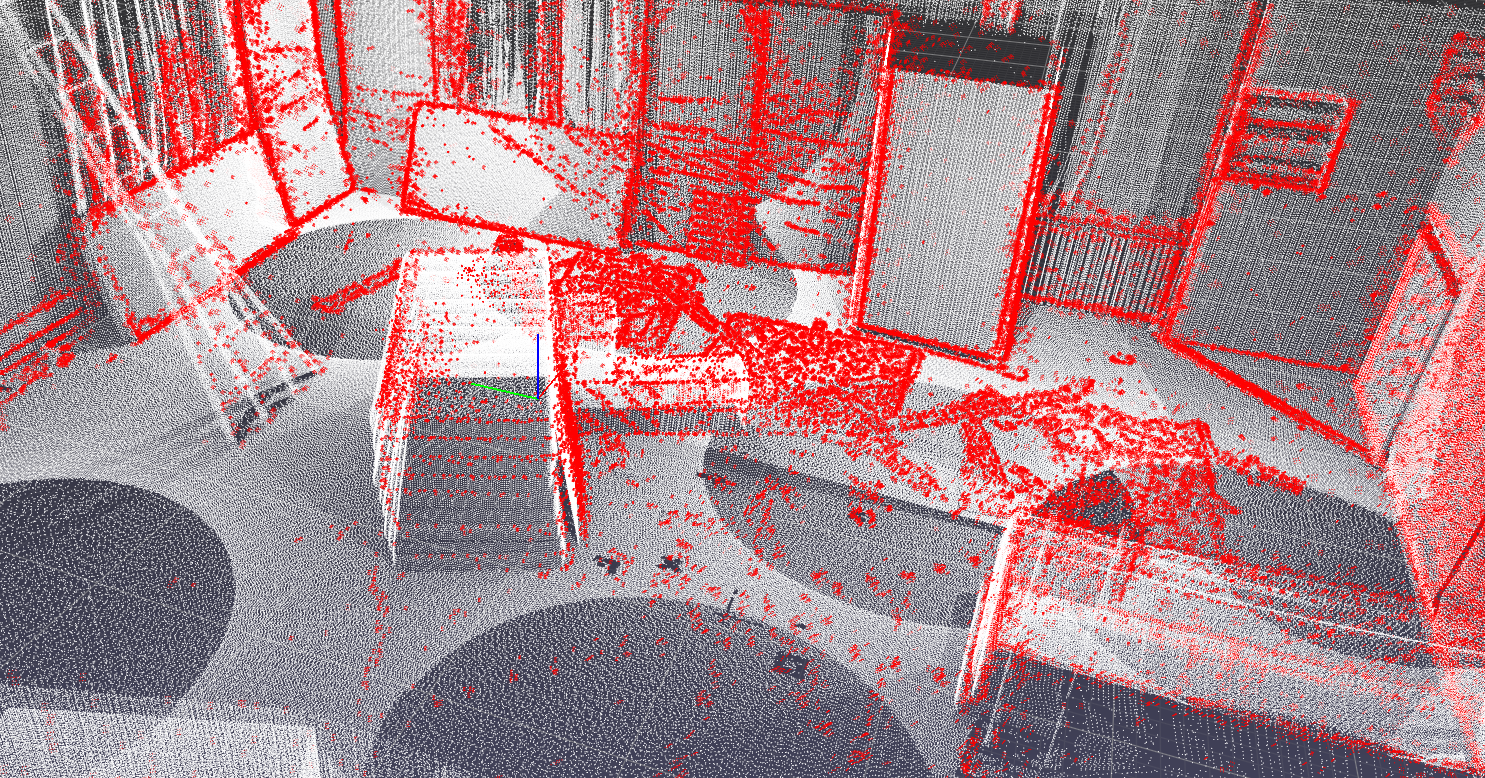
\includegraphics[width=4cm]{img/pointcloud_dsm} }}%
	\qquad
    \subfloat[\centering DSO]{{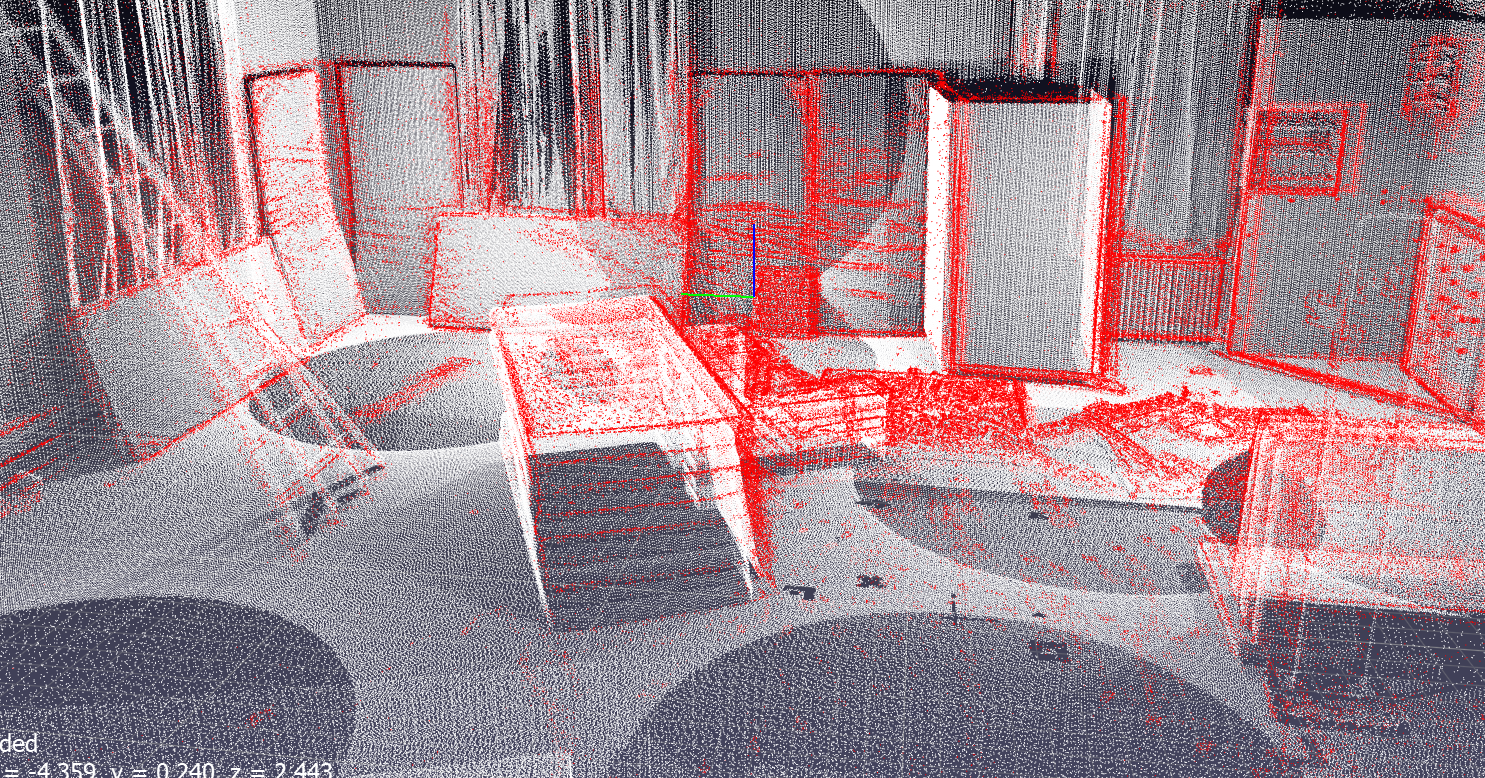
\includegraphics[width=4cm]{img/pointcloud_dso} }}%
    \caption{The groundtruth of the Pointcloud from Sequence V101 (white points) and the evaluated points by each algorithm (red points). 
	The points in Figure (a) are four times as large for better visability (ORB-SLAM generates only few points). 
	}%
    \label{fig:pointcloud}%
	\end{figure}
	
	
	\begin{table}
	\caption{Number and accuracy of evaluated points of each algorithm}
	\begin{tabular}{ |p{3cm}||p{3cm}|p{3cm}|p{3cm}|  }
	\hline
	Sequence Name& ORB & DSM & DSO \\
	\hline
	MH\_01\_easy & 8958 (/) & 675720 (/) & 361633 (/)\\
	MH\_02\_easy & 8692 (/) & 700920 (/) & 343804 (/)\\
	MH\_03\_medium & / (/) & 614264 (/) & 371752 (/)\\
	MH\_04\_difficult & 7943 (/) & 495752 (/) & 208445 (/)\\
	MH\_05\_difficult & 8373 (/) & 517712 (/) & 232415 (/)\\
	V1\_01\_easy & 7075 (0.049) & 6108440 (0.066) & 374257 (0.066)\\
	V1\_02\_medium & 6517 (0.042) & 648440 (0.187) & 366513 (1.458)\\
	V1\_03\_difficult & / (/) & 775080 (0.092) & 448212 (0.459)\\
	V2\_01\_easy & / (/) & 584552 (0.58) & 247905 (0.086)\\
	V2\_02\_medium & / (/)& 733992 (0.078) & 490608 (0.104)\\
	V2\_03\_difficult & / (/) & 921312 (0.645) & 465396 (0.677)\\
	\hline
	\end{tabular}
	\label{table:pointcloud}
	\end{table}
	
	
	\fig{img/pq_dist.png}{Boxplot of the eucleadian distances between an evaluated point and the closest point of the ground truth point cloud.
	For computational feasibility, for each sequence and algorithm, 500 points for evaluation are sampled randomly}{fig:boxplot_pq}{0.8}
	
	

\section{Calculation Time}

	\begin{table}
	\caption{Computation Time (excluded time needed for initialization) of each Sequence and Algorithm}
	\begin{tabular}{ |p{3cm}||p{3cm}|p{3cm}|p{3cm}|  }
	\hline
	Sequence Name& Computation Time in $s$ ORB & Computation Time in $s$ DSM & Computation Time in $s$ DSO \\
	\hline
	MH\_01\_easy & 257 & 1098 & 749\\
	MH\_02\_easy & 209 & 984 & 690\\
	MH\_03\_medium & 198 & 1369 & 707\\
	MH\_04\_difficult & 165 & 896 & 504\\
	MH\_05\_difficult & 193 & 825 & 633\\
	V1\_01\_easy & 253 & 1383 & 905\\
	V1\_02\_medium & 150 & 1550 & 820\\
	V1\_03\_difficult & 186 & 2262 & 1134\\
	V2\_01\_easy & 187 & 1045 & 612\\
	V2\_02\_medium & 162 & 1675 & 1522\\
	V2\_03\_difficult & 143 & 1600 & 793\\
	\hline
	\end{tabular}
	\label{table:comp_time}
	\end{table}

